\chapter{Implementation}
\label{ch:implementation}

\emph{In this section, you should present what you have done. How things have been implemented and how they work.
Please avoid putting lines and lines of code here. But you can highlight some important elements of your implementations (some important part of the code, if necessary).}

\section{Structure of the Simulation}
\emph{Explain why you chose this structure and why you chose these hallucinations and sentences}

The structure of the simulation was carefully designed to evoke a progressively immersive and unsettling representation of hallucinations associated with schizophrenia. This structure was chosen to reflect both phenomenological research on psychotic symptoms and evidence-based educational strategies for increasing empathy and reducing stigma in health professionals.

The auditory hallucinations used in this simulation draw from documented simulation programs such as Patricia Deegan’s “Hearing Voices,” which have been shown to significantly impact empathy levels in students and clinicians \cite{Hsia2022}. In alignment with these findings, the simulation integrates a sequence of whispered voices and confrontational phrases. The sentences were crafted and timed intentionally to gradually escalate in emotional intensity, following research that demonstrates increased affective engagement leads to more powerful learning and emotional responses \cite{Skoy2016}.

Complementing the auditory component are visual hallucination elements, including dynamically spawning colored spheres, spatial distortions through dot placements, and visual darkening of the field of view. These visuals were inspired by clinical descriptions of visual hallucinations in psychotic disorders, such as geometric distortions, flickering lights, and anthropomorphic or symbolic figures \cite{Silverstein2021,Vanommen2019}.

The structural design aims to simulate both simple and complex hallucinations. Early stimuli (whispers, darkness) mimic the subtle onset of perceptual anomalies, while the crescendo of auditory cues and visual manifestations evoke the overwhelming nature of full-blown psychosis. This approach allows users to move from discomfort to disorientation, simulating the lived experience of progressive symptom development.

\section{Implementation of the Simulation}
\emph{Explain how you implemented the simulation. What are the main components of the simulation? How do they interact with each other?}
The simulation was implemented in Unity and constructed through modular components that interact in time-dependent sequences coordinated by a central control script.

\subsection{Orchestration}
At the heart of the system lies the \textit{Orchestrator.cs} script. This script sequences the entire simulation, controlling when sounds play, visual hallucinations appear, and environmental effects occur. The timeline was structured using IEnumerator coroutines, allowing asynchronous timed execution of events, ensuring immersive pacing without overwhelming the user too early in the experience.

Synchronization across components ensures the user is not overwhelmed with concurrent stimuli too early. For example, whispers begin before visuals, allowing users to acclimate to auditory disturbances before confronting the more jarring visual phenomena. Visual hallucinations are also paced in relation to emotional escalation in the voice samples, building tension across the timeline.

\begin{figure}[h!]
    \centering
    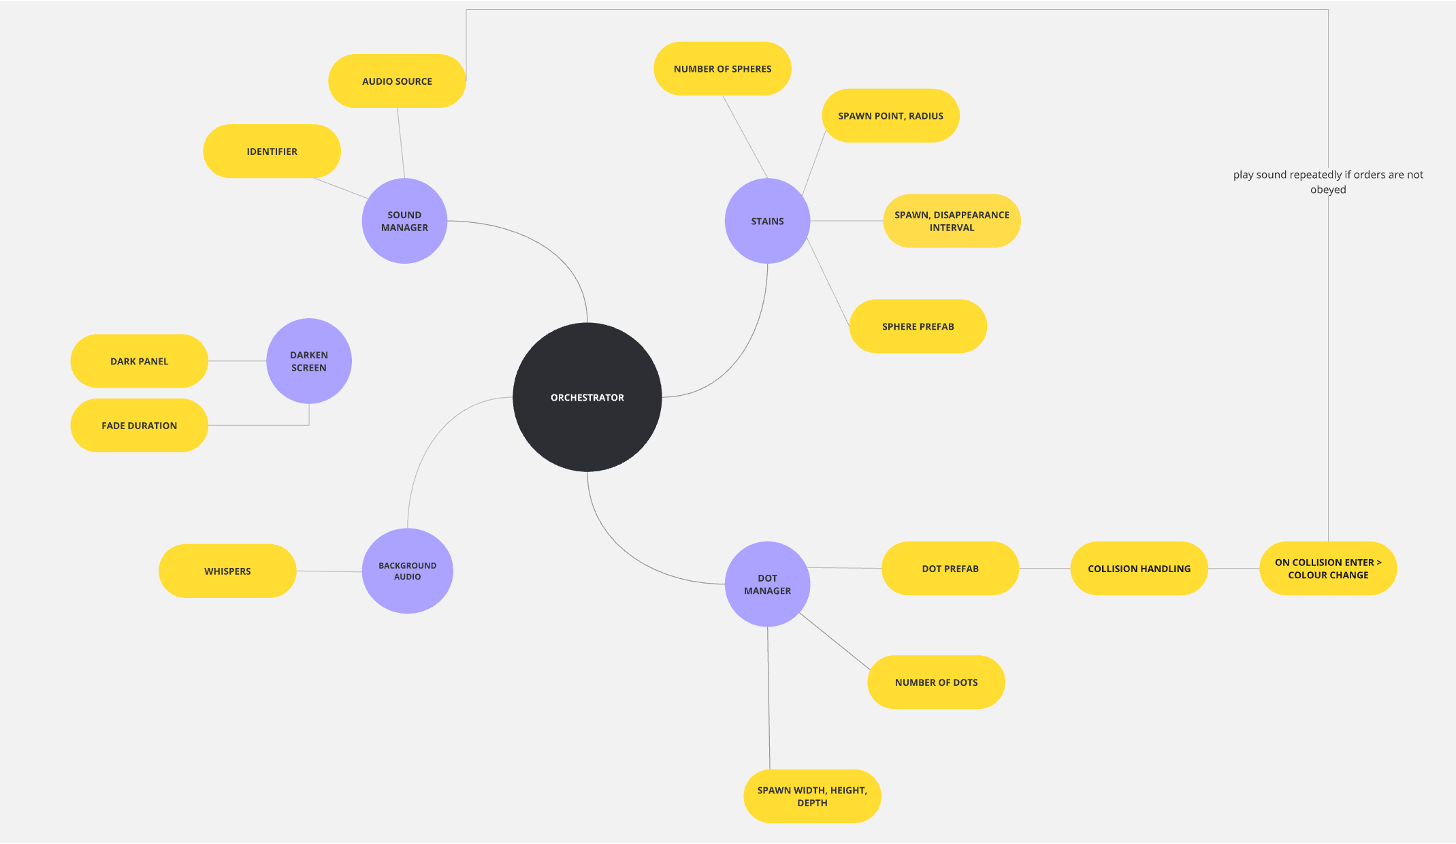
\includegraphics[width=0.8\textwidth]{../../Figures/Orch-sequence.png}
    \caption{Diagram of the Orchestrator system showing the interaction between auditory, visual, and environmental components.}
    \label{fig:orchestrator}
\end{figure}


\begin{landscape}
    \begin{center}
    \resizebox{\textwidth}{!}{ 
    \begin{tikzpicture}[node distance=1.5cm and 2.5cm, every node/.style={font=\small}]
    \tikzset{
      block/.style={rectangle, draw=black, fill=yellow!50, rounded corners, minimum height=1.2em, text centered, text width=3.2cm},
      module/.style={circle, draw=black, fill=blue!30, minimum size=2cm, text centered, align=center},
      orchestrator/.style={circle, draw=black, fill=black, text=white, minimum size=2.5cm, text centered},
      arrow/.style={-Stealth, thick}
    }
    
    % Central node
    \node[orchestrator] (orchestrator) {ORCHESTRATOR};
    
    % Top-left: SOUND MANAGER
    \node[module, above left=5cm and 2.5cm of orchestrator] (sound) {SOUND\\MANAGER};
    \node[block, above=of sound] (audio) {AUDIO SOURCE};
    \node[block, left=of sound] (identifier) {IDENTIFIER};
    \draw[arrow] (orchestrator) -- (sound);
    \draw[arrow] (audio) -- (sound);
    \draw[arrow] (identifier) -- (sound);
    
    % Top-right: STAINS
    \node[module, above right=5cm and 2.5cm of orchestrator] (stains) {STAINS};
    \node[block, above=of stains] (spawnpoint) {SPAWN POINT, RADIUS};
    \node[block, right=of stains] (numspheres) {NUMBER OF SPHERES};
    \node[block, below=of stains] (interval) {SPAWN, DISAPPEARANCE INTERVAL};
    \node[block, below left=of stains] (sphereprefab) {SPHERE PREFAB};
    \draw[arrow] (orchestrator) -- (stains);
    \draw[arrow] (spawnpoint) -- (stains);
    \draw[arrow] (numspheres) -- (stains);
    \draw[arrow] (interval) -- (stains);
    \draw[arrow] (sphereprefab) -- (stains);
    
    % Bottom-right: DOT MANAGER
    \node[module, below right=4cm and 2.5cm of orchestrator] (dot) {DOT\\MANAGER};
    \node[block, right=of dot] (dotprefab) {DOT PREFAB};
    \node[block, below=of dotprefab] (collision) {COLLISION HANDLING};
    \node[block, below=of collision] (colorchange) {ON COLLISION ENTER > COLOUR CHANGE};
    \node[block, below=of dot] (numdots) {NUMBER OF DOTS};
    \node[block, left=of numdots] (spawndims) {SPAWN WIDTH, HEIGHT, DEPTH};
    \draw[arrow] (orchestrator) -- (dot);
    \draw[arrow] (dotprefab) -- (dot);
    \draw[arrow] (collision) -- (dotprefab);
    \draw[arrow] (colorchange) -- (collision);
    \draw[arrow] (numdots) -- (dot);
    \draw[arrow] (spawndims) -- (dot);
    
    % Bottom-center: BACKGROUND AUDIO
    \node[module, below=5cm of orchestrator] (background) {BACKGROUND\\AUDIO};
    \node[block, left=of background] (whispers) {WHISPERS};
    \draw[arrow] (orchestrator) -- (background);
    \draw[arrow] (whispers) -- (background);
    
    % Bottom-left: DARKEN SCREEN
    \node[module, below left=4cm and 2.5cm of orchestrator] (darken) {DARKEN\\SCREEN};
    \node[block, left=of darken] (darkpanel) {DARK PANEL};
    \node[block, below=of darkpanel] (fadeduration) {FADE DURATION};
    \draw[arrow] (orchestrator) -- (darken);
    \draw[arrow] (darkpanel) -- (darken);
    \draw[arrow] (fadeduration) -- (darken);
    
    % Note repositioned far top right
    \node[block, right=8.5cm of orchestrator, text width=4cm, align=left, font=\itshape\small] (note) {Play sound repeatedly if orders are not obeyed};
    \draw[->, dashed] (note.west) to[bend right=20] (stains.east);
    
    \end{tikzpicture}
    }
    \end{center}
    \end{landscape}
    

    \subsection{Auditory Hallucinations}

    The auditory effects in the system are handled by the \textit{SoundManager.cs} script. Audio files are grouped by voice type, making it easy to play back different kinds of hallucination samples. These voices include phrases that sound accusatory, confusing, or frightening—reflecting common real-world descriptions of auditory hallucinations.
    
    The voices were generated using ElevenLabs, a text-to-speech AI engine \cite{elevenlabs}. Each one was created with a specific emotional tone in mind: one voice sounds scared and almost shouting, another is snooty and mean, and the third sounds lost and desperate. These voices are played at key moments to create a stronger sense of fear, confusion, or paranoia. Their timing is matched with visual effects to create a more immersive and realistic experience of multisensory hallucinations.
    
    In addition, the \textit{ObjectCollision.cs} script adds interactive audio that loops until the user physically interacts with an object. This mimics the frustrating and unpredictable nature of hallucinations, as often described by people experiencing psychosis.
    
    

\subsection{Visual Hallucinations}
Visual components are diversified to simulate various hallucination types:
\begin{itemize}
    \item Wave Deformation: \textit{DynamicWaveDeformation.cs} distorts object surfaces using transformations, creating a pulsating geometry that mimics perceptual distortions in psychosis.
    \item Gradual Screen Darkening: \textit{ScreenDarkener.cs} overlays a semi-transparent black UI panel to simulate the narrowing of visual perception or "tunnel vision," often reported during intense hallucinations.
    \item Dot Fields: \textit{DotManager.cs} creates random red and blue dots that appear above the user. These dots represent chaotic visual input or visual noise, similar to the floating patterns often described by people experiencing psychosis.
    \item Pulsating Spheres: The Orchestrator periodically spawns spherical objects, creating a feeling of presence and spatial invasion. Their randomness and impermanence reflect transient hallucinations and visual object anomalies.
\end{itemize}

Each visual element in the system was designed based on descriptions of how people with schizophrenia may experience their symptoms. These experiences are often grouped into simple, geometric, and complex visual types \cite{Silverstein2021,Vanommen2019}.

The way the system is built makes it easy to expand in the future.